\documentclass[10pt]{report}

\usepackage{stan-talks}

\begin{document}

\sf
\vspace*{6pt}
\noindent
\spc{\huge\bfseries \color{MidnightBlue}{Section 4.}
\\[8pt]
\spc{\Huge\bfseries \color{MidnightBlue}{How Stan Works}}}
\vfill
\noindent
\spc{\large\bfseries Bob Carpenter}
\\[4pt]
\spc{Columbia University}
\vfill
\hfill 

\mypart{Part I}{What Stan Does}

\sld{Full Bayes: No-U-Turn Sampler}

\begin{itemize}
\item Adaptive \myemph{Hamiltonian Monte Carlo} (HMC)
\begin{subitemize}
\item \myemph{Potential Energy}: negative log posterior
\item \myemph{Kinetic Energy}: random standard normal per iteration
\end{subitemize}
  % 
\item Adaptation \myemph{during warmup}
  \vspace*{-4pt}
  \begin{itemize}\small
  \item step size adapted to target total acceptance rate
  \item mass matrix estimated with regularization
  \end{itemize}
  % 
\item Adaptation \myemph{during sampling}
  \begin{subitemize}
  \item simulate forward and backward in time until U-turn
  \end{subitemize}
  % 
\item \myemph{Slice sample} along path
% \item \myemph{Initialization} user-specified or random unconstrained
\vfill
\hfill 
{\footnotesize (Hoffman and Gelman 2011, 2014)}
\end{itemize}


\sld{Posterior Inference}

\begin{itemize}
\item Generated quantities block for \myemph{inference}
  \\ {\footnotesize (predictions, decisions, and event probabilities)}
\item \myemph{Extractors} for draws in sample in RStan and PyStan
\item Coda-like \myemph{posterior summary}
  \vspace*{-4pt}
  \begin{itemize}\small
  \item posterior mean w.\ MCMC std.\ error, std.\ dev., quantiles
  \item split-$\hat{R}$ multi-chain convergence diagnostic (Gelman/Rubin)
  \item multi-chain effective sample size estimation (FFT algorithm)
  \end{itemize}
\item Model comparison with \myemph{WAIC}
\begin{subitemize}
\item in-sample approximation to cross-validation
\end{subitemize}
\end{itemize}

\sld{Penalized MLE}

\begin{itemize}
\item Posterior \myemph{mode finding} via L-BFGS optimization
  \\ {\footnotesize (uses model gradient, efficiently approximates Hessian)}
\item \myemph{Disables Jacobians} for parameter inverse transforms
  \item  \myemph{Standard errors} on unconstrained scale
    \\
    {\footnotesize  (estimated using curvature of penalized log likelihood function}
\item Models, data, initialization as in MCMC
  \vfill
\item \myemph{Very Near Future}
  \vspace*{-4pt}
  \begin{itemize}\small
  \item Standard errors \myemph{on constrained scale}
    \\
    {\footnotesize  (sample unconstrained approximation and inverse transform)}
  \end{itemize}      
\end{itemize}

\sld{``Black Box'' Variational Inference}
\begin{itemize}
%
\item \myemph{Black box} so can fit any Stan model
%
\item Multivariate \myemph{normal approx to unconstrained} posterior
\begin{subitemize}
\item covariance: diagonal mean-field or full rank
\item not Laplace approx --- around posterior mean, not mode
\item transformed back to constrained space (built-in Jacobians)
\end{subitemize}
%
\item Stochastic \myemph{gradient-descent} optimization
\begin{subitemize}
\item ELBO gradient estimated via Monte Carlo + autdiff
\end{subitemize}
%
\item Returns \myemph{approximate posterior} mean / covariance
\item Returns \myemph{sample} transformed to constrained space
\end{itemize}

\sld{Posterior Analysis: Estimates}
\begin{itemize}
\item For each parameter (and \code{lp\_\_})
\begin{subitemize}
\item Posterior mean
\item Posterior standard deviation
\item Posterior MCMC error esimate:  $\mbox{sd} / N_{\mathrm{eff}}$
\item Posterior quantiles
\item Number of effective samples
\item $\hat{R}$ convergence statistic
\end{subitemize}
\vfill
\item \ldots and much much more in ShinyStan
\end{itemize}

\sld{Stan as a Research Tool}
\begin{itemize}
\item Stan can be used to \myemph{explore algorithms}
\item Models transformed to \myemph{unconstrained support} on $\mathbb{R}^n$
\item Once a model is compiled, have
  \vspace*{-4pt}
  \begin{itemize}\small
  \item \myemph{log probability, gradient} \hfill (soon: Hessian)
  \item data I/O and parameter initialization
  \item model provides variable names and dimensionalities
  \item transforms to and from constrained representation 
    \\ {\footnotesize (with or without Jacobian)}
  \end{itemize}
\end{itemize}


\mypart{Part II}{How Stan Works}

\sld{Model: Read and Transform Data}
\begin{itemize}
\item Only done once for optimization or sampling (per chain)
\item Read data
\begin{subitemize}
\item read data variables from memory or file stream
\item validate data
\end{subitemize}
\item Generate transformed data
\begin{subitemize}
\item execute transformed data statements
\item validate variable constraints when done
\end{subitemize}
\end{itemize}

\sld{Model: Log Density}
\begin{itemize}
\item \emph{Given} parameter values on unconstrained scale
\item Builds expression graph for log density (start at 0)
\item Inverse transform parameters to constrained scale
\begin{subitemize}
\item constraints involve non-linear transforms
\item e.g.,  positive constrained $x$ to unconstrained $y = \log x$
\end{subitemize}
\item account for curvature in change of variables
\begin{subitemize}
\item e.g., unconstrained $y$ to positive $x = \log^{-1}(y) =
  \exp(y)$
\item e.g., add log Jacobian determinant, $\log |\frac{d}{dy} \exp(y)| = y$
\end{subitemize}
\item Execute model block statements to increment log density
\end{itemize}

\sld{Model: Log Density Gradient}
\begin{itemize}
\item Log density evaluation builds up expression graph
\begin{subitemize}
\item templated overloads of functions and operators
\item efficient arena-based memory management
\end{subitemize}
\item Compute gradient in backward pass on expression graph 
\begin{subitemize}
\item propagate partial derivatives via chain rule
\item work backwards from final log density to parameters
\item dynamic programming for shared subexpressions
\end{subitemize}
\item Linear multiple of time to evalue log density
\end{itemize}

\sld{Model: Generated Quantities}
\begin{itemize}
\item \myemph{Given} parameter values
\item Once per iteration (not once per leapfrog step)
\item May involve (pseudo) random-number generation
\begin{subitemize}
\item Executed generated quantity statements
\item Validate values satisfy constraints
\end{subitemize}
\item Typically used for 
\begin{subitemize}
\item Event probability estimation
\item Predictive posterior estimation
\end{subitemize}
\item Efficient because evaluated with \code{double} types (no autodiff)
\end{itemize}

\sld{Optimize: \ L-BFGS}
\vspace*{-4pt}
\begin{itemize}
\item Initialize unconstrained parameters and Hessian
\begin{subitemize}
\item Random values on unconstrained scale uniform in $(-2,2)$
\begin{subsubitemize}
\item or user specified on constrained scale, transformed
\end{subsubitemize}
\item Hessian approximation initialized to unit matrix
\end{subitemize}
\item While not converged
\begin{subitemize}
\item Move unconstrained parameters toward optimum based on Hessian approximation and
  step size (Newton step)
\item If diverged (arithmetic, support), reduce step size, continue
\item else if converged (parameter change, log density change, gradient
  value), return value
\item else update Hessian approx. based on calculated gradient
\end{subitemize}
\end{itemize}

\sld{Sample: Hamiltonian Flow}
\vspace*{-4pt}
\begin{itemize}
\item Generate random \myemph{kinetic energy} 
\vspace*{-2pt}
\begin{subitemize}
\item random $\distro{Normal}(0,1)$ in each parameter
\end{subitemize}
\item Use negative log posterior as \myemph{potential energy}
\item Hamiltonian is kinetic plus potential energy
\item \myemph{Leapfrog Integration}: for \emph{fixed} stepsize (time discretization), number of
  steps (total time), and mass matrix,
\begin{subitemize}
\item update momentum half-step based on potential (gradient)
\item update position full step based on momentum
\item update momentum half-step based on potential
\end{subitemize}
\footnotesize
\item Numerical solution of Hamilton's first-order version of
  Newton's second-order diff-eqs of motion ($\mbox{force} =
  \mbox{mass} \times \mbox{acceleration}$)
\end{itemize}

\sld{Sample: Leapfrog Example}
\begin{center}
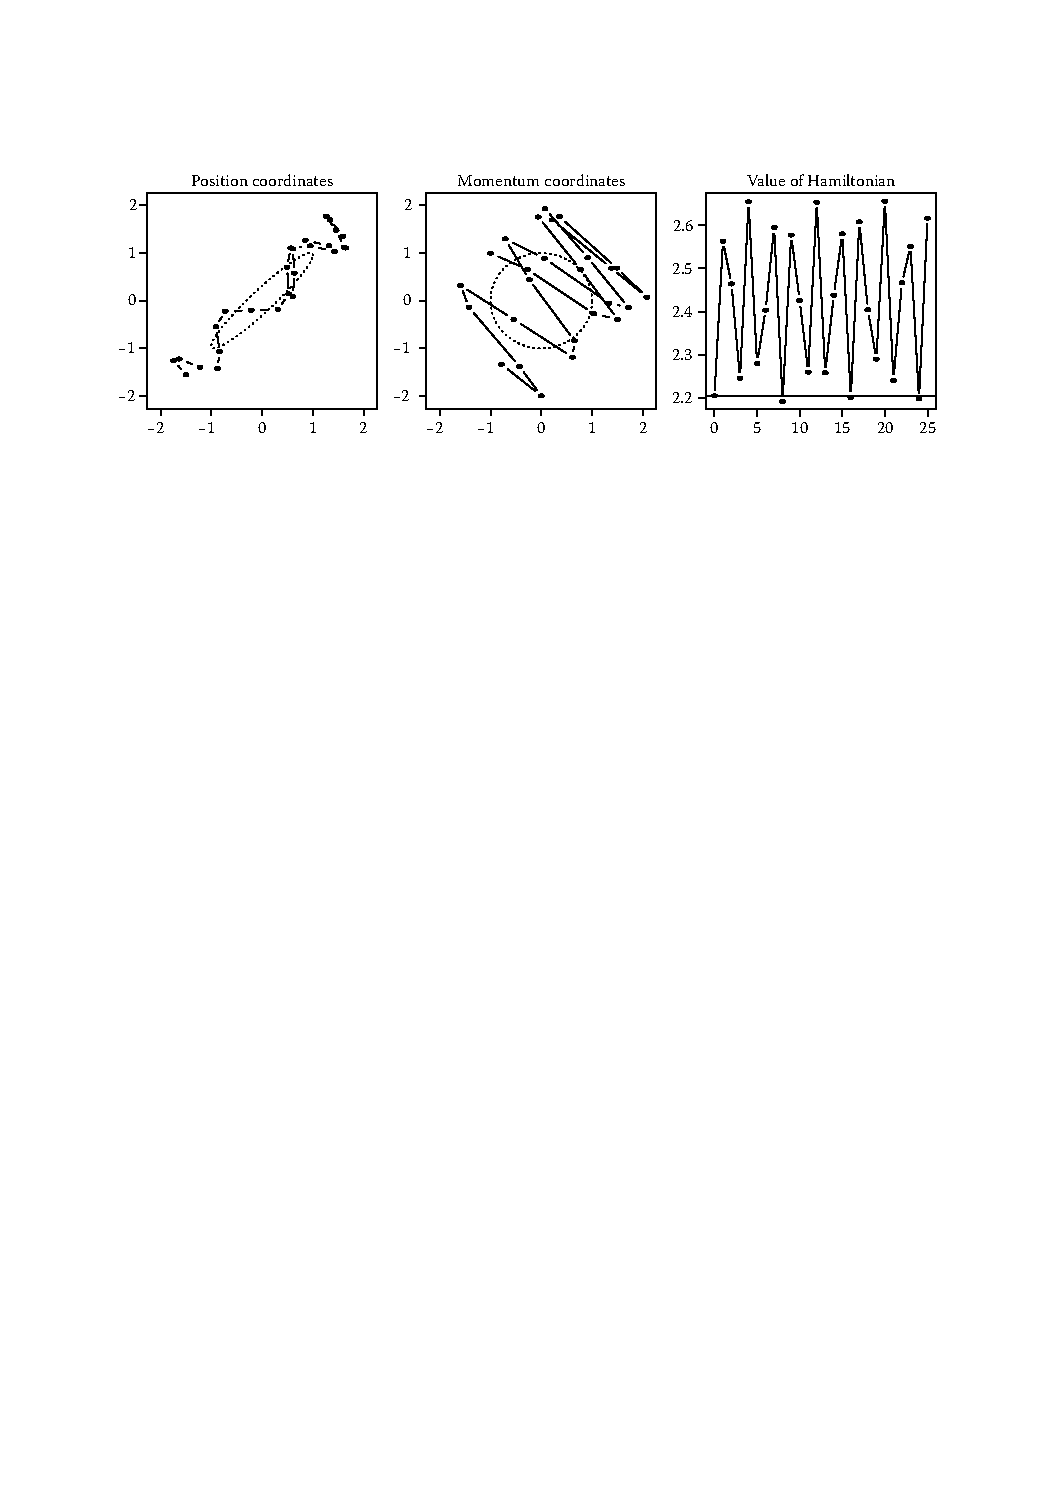
\includegraphics[width=0.9\textwidth]{img/neal-leapfrog.pdf}
\end{center}
\vspace*{-8pt}
\begin{subitemize}
\item \small Trajectory of 25 leapfrog steps for correlated 2D normal (ellipses at 1 sd
  from mean), stepsize of 0.25, initial state of $(-1,1)$, and initial
  momentum of $(-1.5,-1.55)$.  
\\[12pt]
\footnotesize Radford Neal (2013) MCMC using Hamiltonian Dynamics. In {\slshape Handbook
of MCMC}. (free online at \url{http://www.mcmchandbook.net/index.html})
\end{subitemize}


\sld{Sample: No-U-Turn Sampler (NUTS)}
\begin{itemize}
\item Adapts Hamiltonian simulation time
\begin{subitemize}
\item goal to maximize mixing, maintaining detailed balance
\item too short devolves to random walk
\item too long does extra work (i.e., orbits)
\end{subitemize}
\item For exponentially increasing number of steps up to max
\begin{subitemize}
\item Randomly choose to extend forward or backward in time
\item Move forward or backward in time number of steps
\begin{subsubitemize}
\item stop if any subtree (size 2, 4, 8, ...) makes U-turn
\item remove all current steps if subtree U-turns (not ends)
\end{subsubitemize}
\end{subitemize}
\item Randomly select param with density above slice (or reject)
\end{itemize}

\sld{Sample: NUTS Binary Tree}
\vspace*{-6pt}
\begin{center}
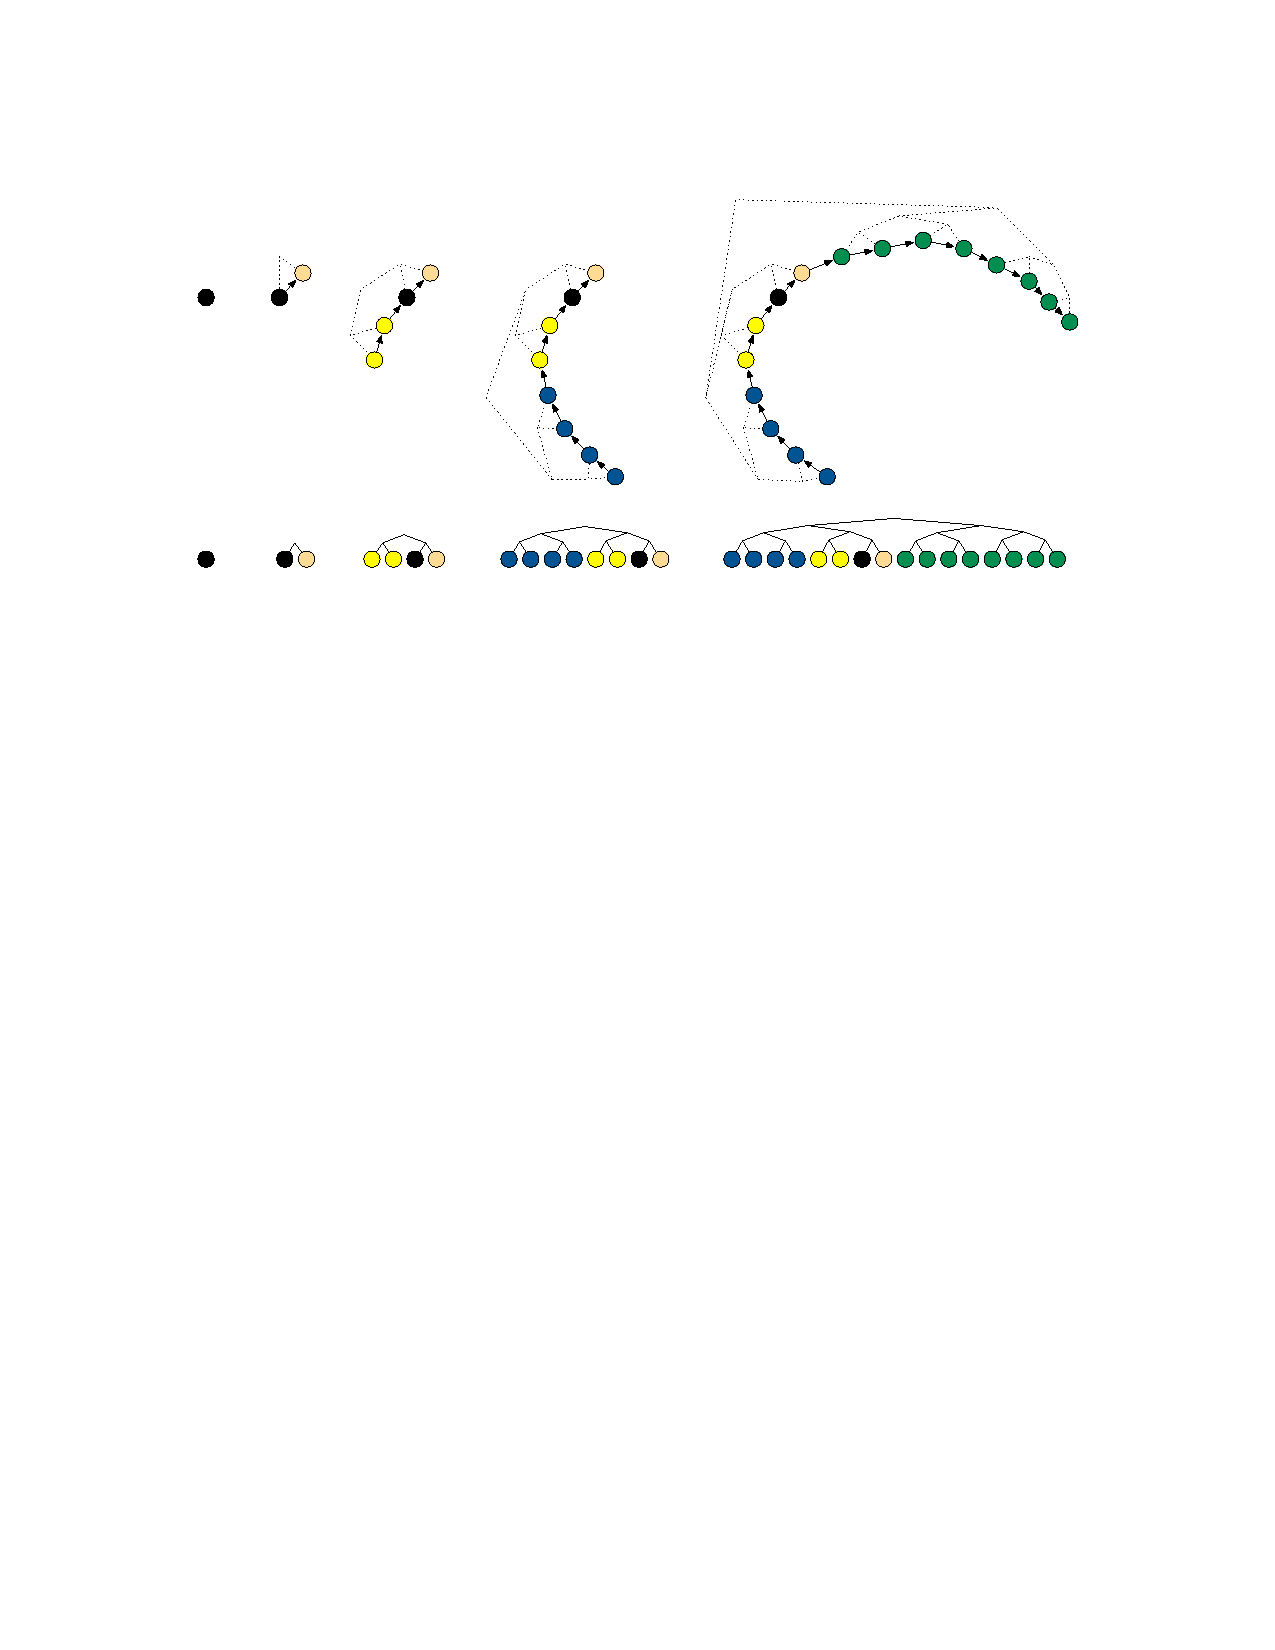
\includegraphics[width=0.9\textwidth]{img/NUTS-tree-evolution.pdf}
\end{center}
\begin{subitemize}
\item Example of repeated doubling building binary tree forward and
  backward in time until U-turn.  
\\[3pt]
\footnotesize
Hoffman and Gelman. 2014. The No-U-Turn Sampler. {\slshape JMLR}.
(free online at \url{http://jmlr.org/papers/v15/hoffman14a.html})
\end{subitemize}

\sld{Sample: NUTS U-Turn}
\\[4pt]
\hspace*{8pt}
\begin{minipage}{0.65\textwidth}
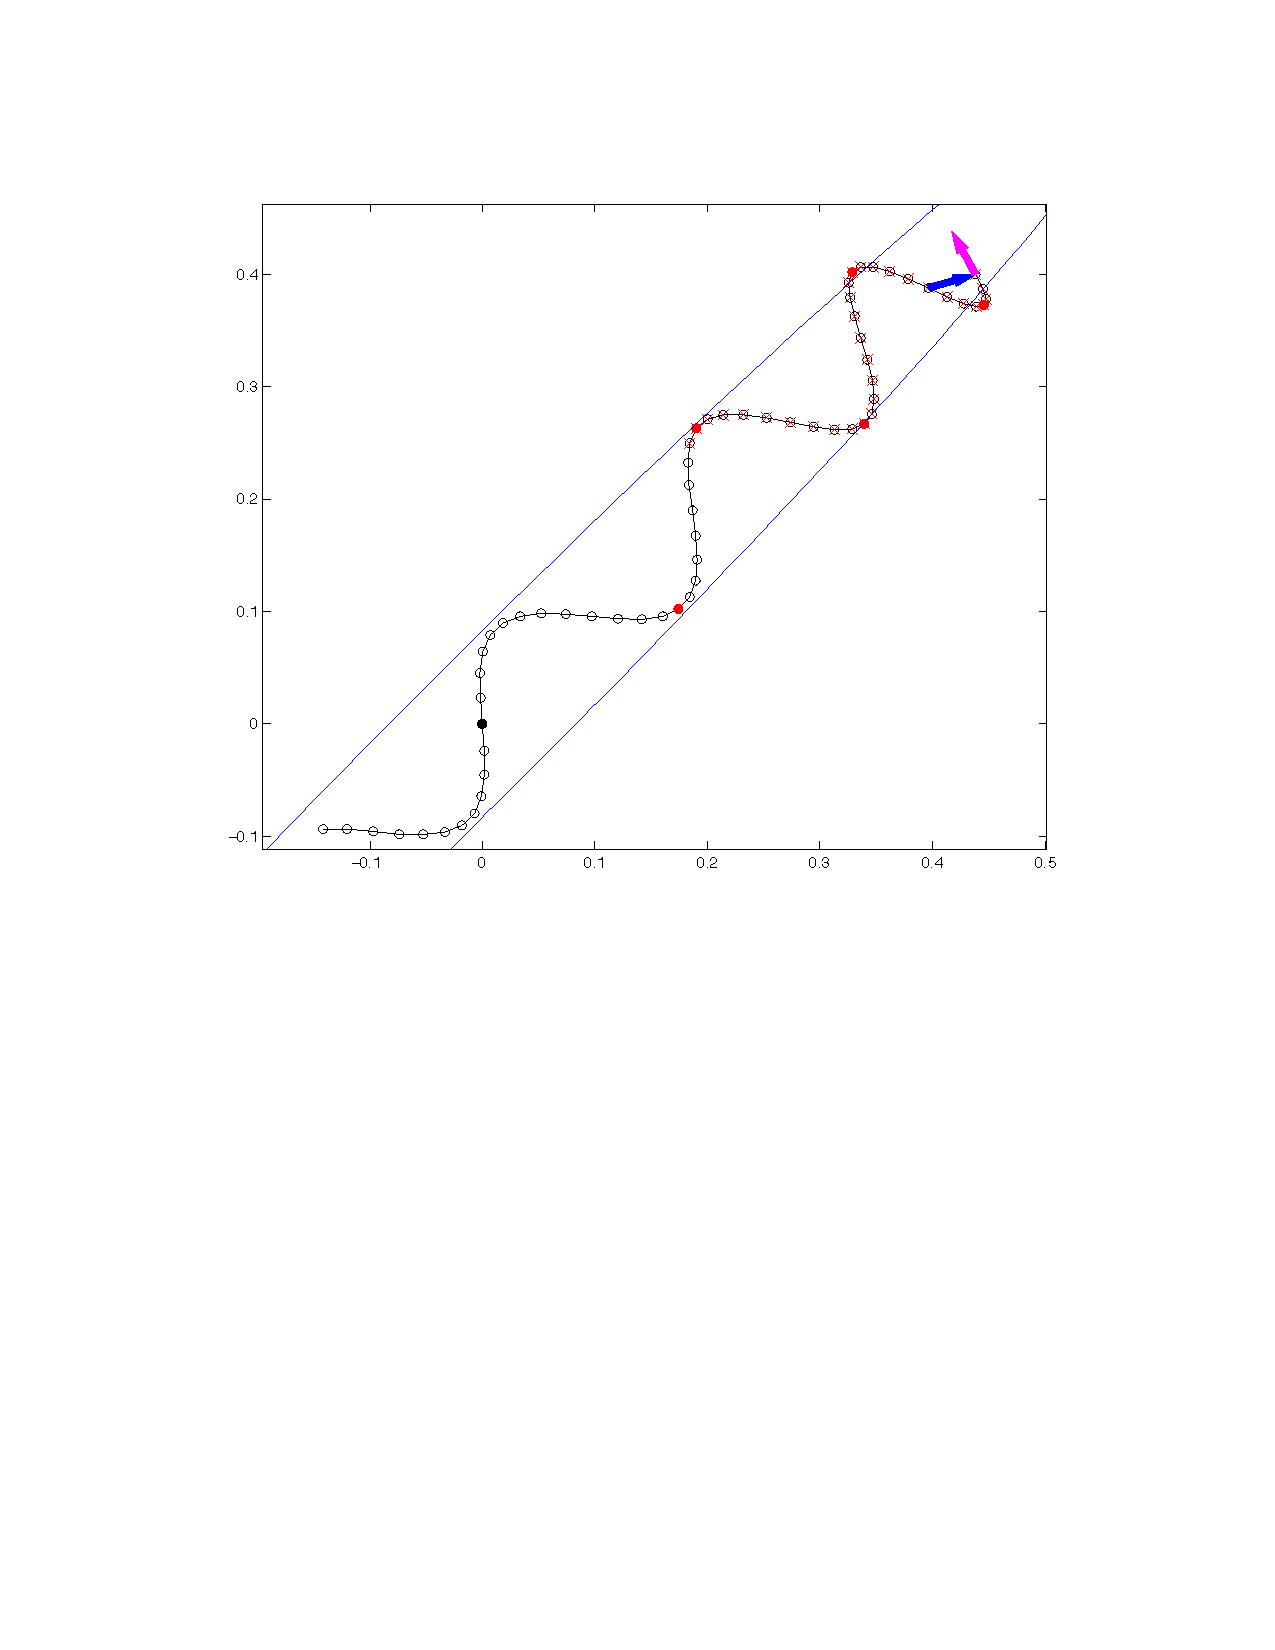
\includegraphics[width=\textwidth]{img/NUTS-trajectory.pdf}
\end{minipage}
\hspace*{-24pt}
\begin{minipage}{0.35\textwidth}
\footnotesize
\begin{subsubitemize}
\item Example of trajectory from one iteration of NUTS.
\item Blue ellipse
  is contour of 2D normal.  
\item Black circles are leapfrog steps.
\item Solid red circles excluded below slice
\item U-turn made with blue and magenta
  arrows
\item  Red crossed circles excluded for detailed balance
\end{subsubitemize}
\end{minipage}

\sld{Sample: HMC/NUTS Warmup}
\begin{itemize}
\item Estimate stepsize 
\begin{subitemize}
\item too small requires too many leapfrog steps
\item too large induces numerical inaccuracy
\item need to balance
\end{subitemize}
\item Estimate mass matrix
\begin{subitemize}
\item Diagonal accounts for parameter scales
\item Dense optionally accounts for rotation
\end{subitemize}
\end{itemize}


\sld{Sample: Warmup (cont.)}
\begin{itemize}
\item Initialize unconstrained parameters as for optimization
\item For exponentially increasing block sizes
\begin{subitemize}
\item for each iteration in block
%
\begin{subsubitemize}
\item generate random kinetic energy
\item simulate Hamiltonian flow (HMC fixed time, NUTS adapts)
\item choose next state (Metroplis for HMC, slice for NUTS)
\end{subsubitemize}
%
\item update regularized point estimate of mass matrix
\begin{subsubitemize}
\item use parameter draws from current block
\item shrink diagonal toward unit; dense toward diagonal
\end{subsubitemize}
\item tune stepsize (line search) for target acceptance rate
\end{subitemize}
\end{itemize}

\sld{Sample: HMC/NUTS Sampling}
\begin{itemize}
\item Fix stepsize and and mass matrix
\item For sampling iterations
\begin{subitemize}
\item generate random kinetic energy
\item simulate Hamiltonian flow
\item apply Metropolis accept/reject (HMC) or slice (NUTS)
\end{subitemize}
\end{itemize}

\sld{NUTS vs.\ Gibbs and Metropolis}

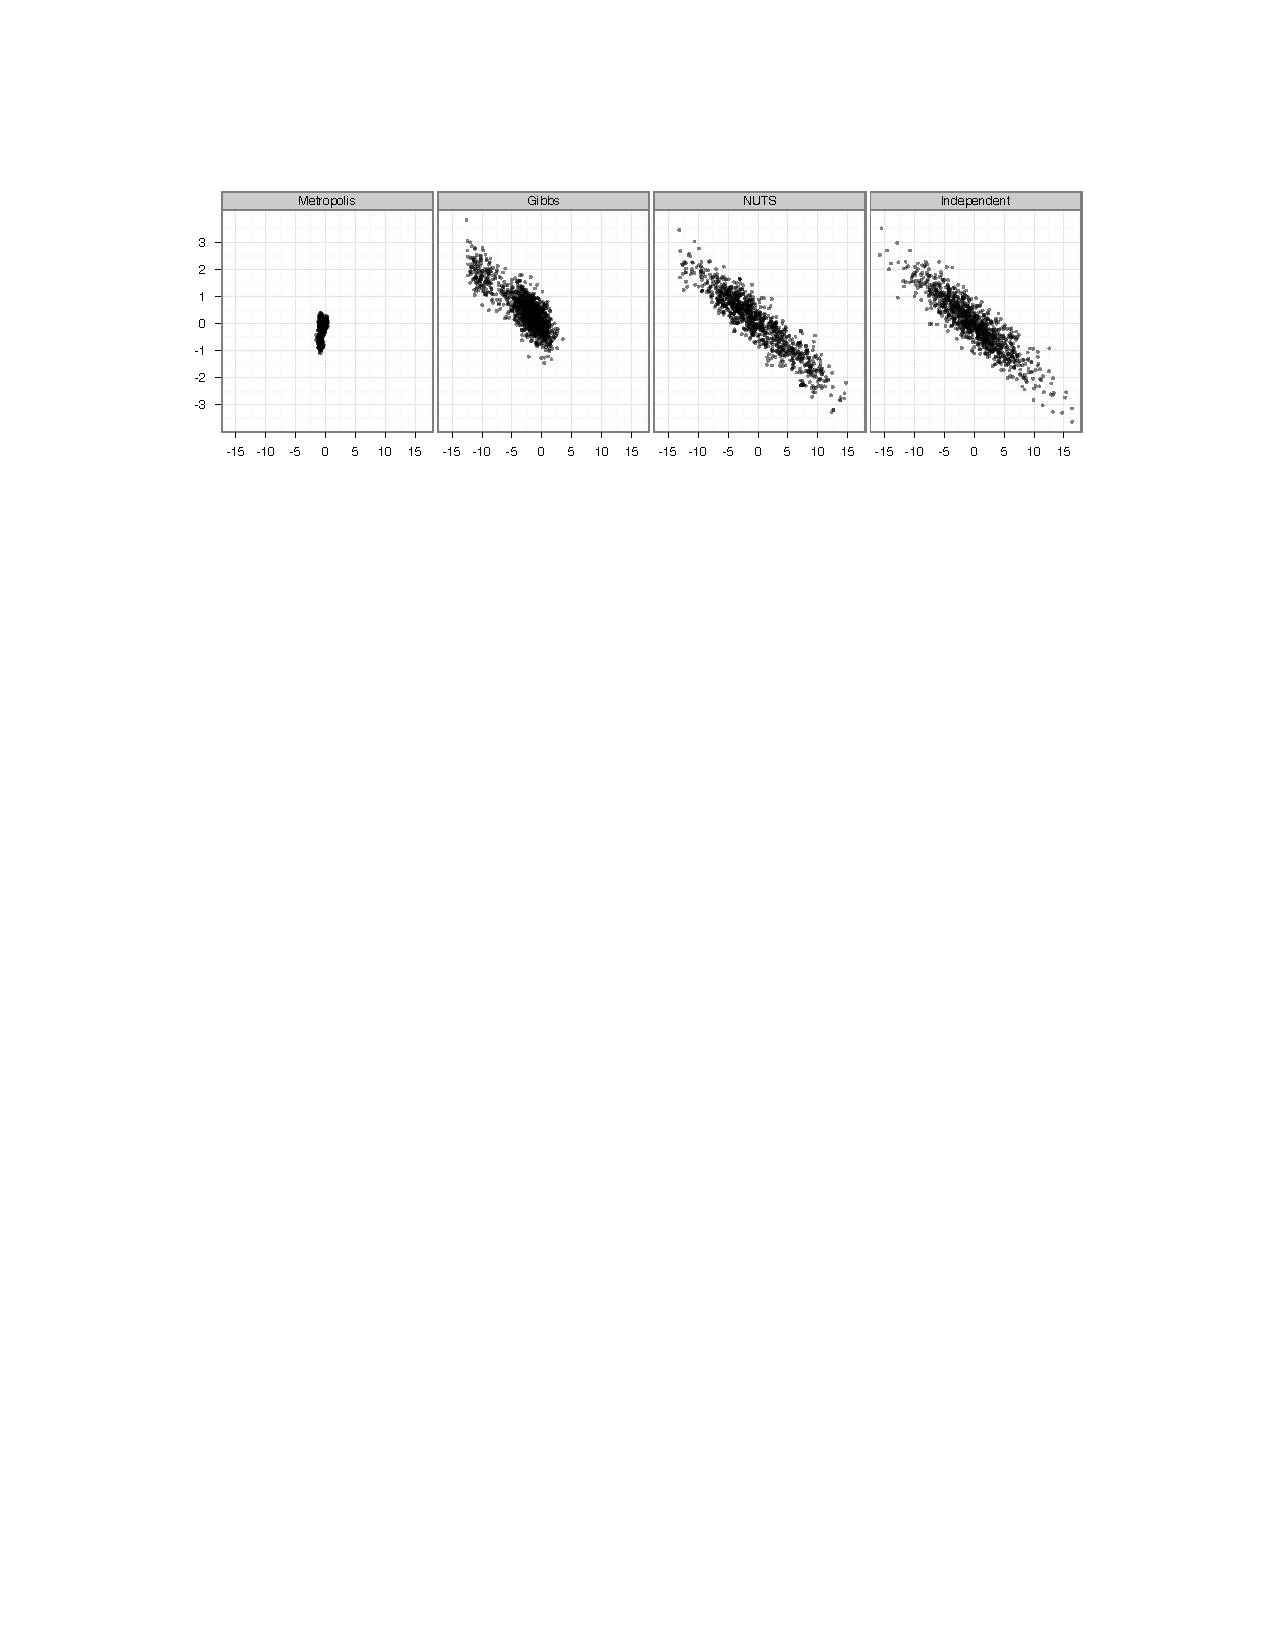
\includegraphics[width=0.9\textwidth]{img/nuts-vs.pdf}
\begin{subitemize}
\item Two dimensions of highly correlated 250-dim normal
\item \myemph{1,000,000 draws} from Metropolis and Gibbs (thin to 1000)
\item \myemph{1000 draws} from NUTS; 1000 independent draws
\end{subitemize}

\sld{NUTS vs.\ Basic HMC}

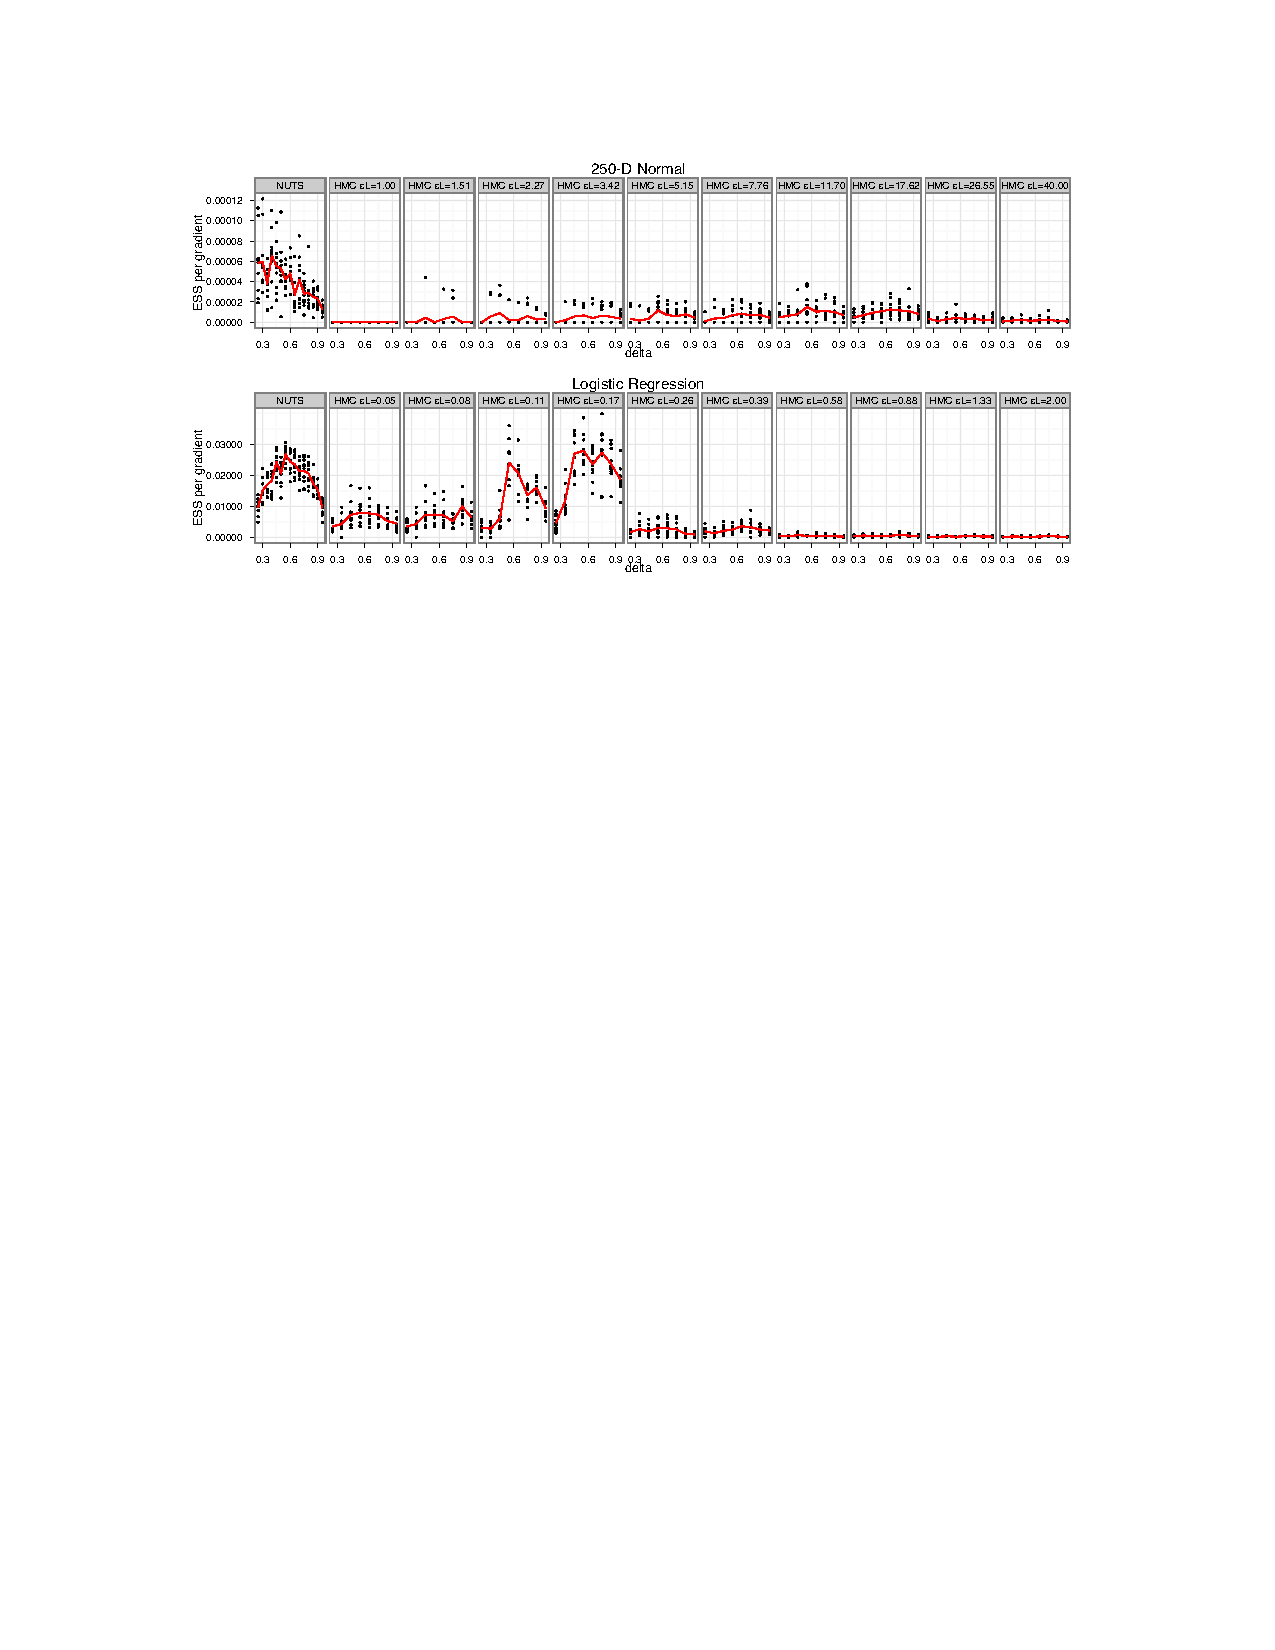
\includegraphics[width=0.9\textwidth]{img/nuts-ess-1.pdf}
{\small
  \begin{itemize}
  \item 250-D normal and logistic regression models
  \item Vertical axis is effective sample size per sample (bigger better)
  \item Left) NUTS; \ \ Right) HMC with increasing $t = \epsilon L$
  \end{itemize}
}

\sld{NUTS vs.\ Basic HMC II}

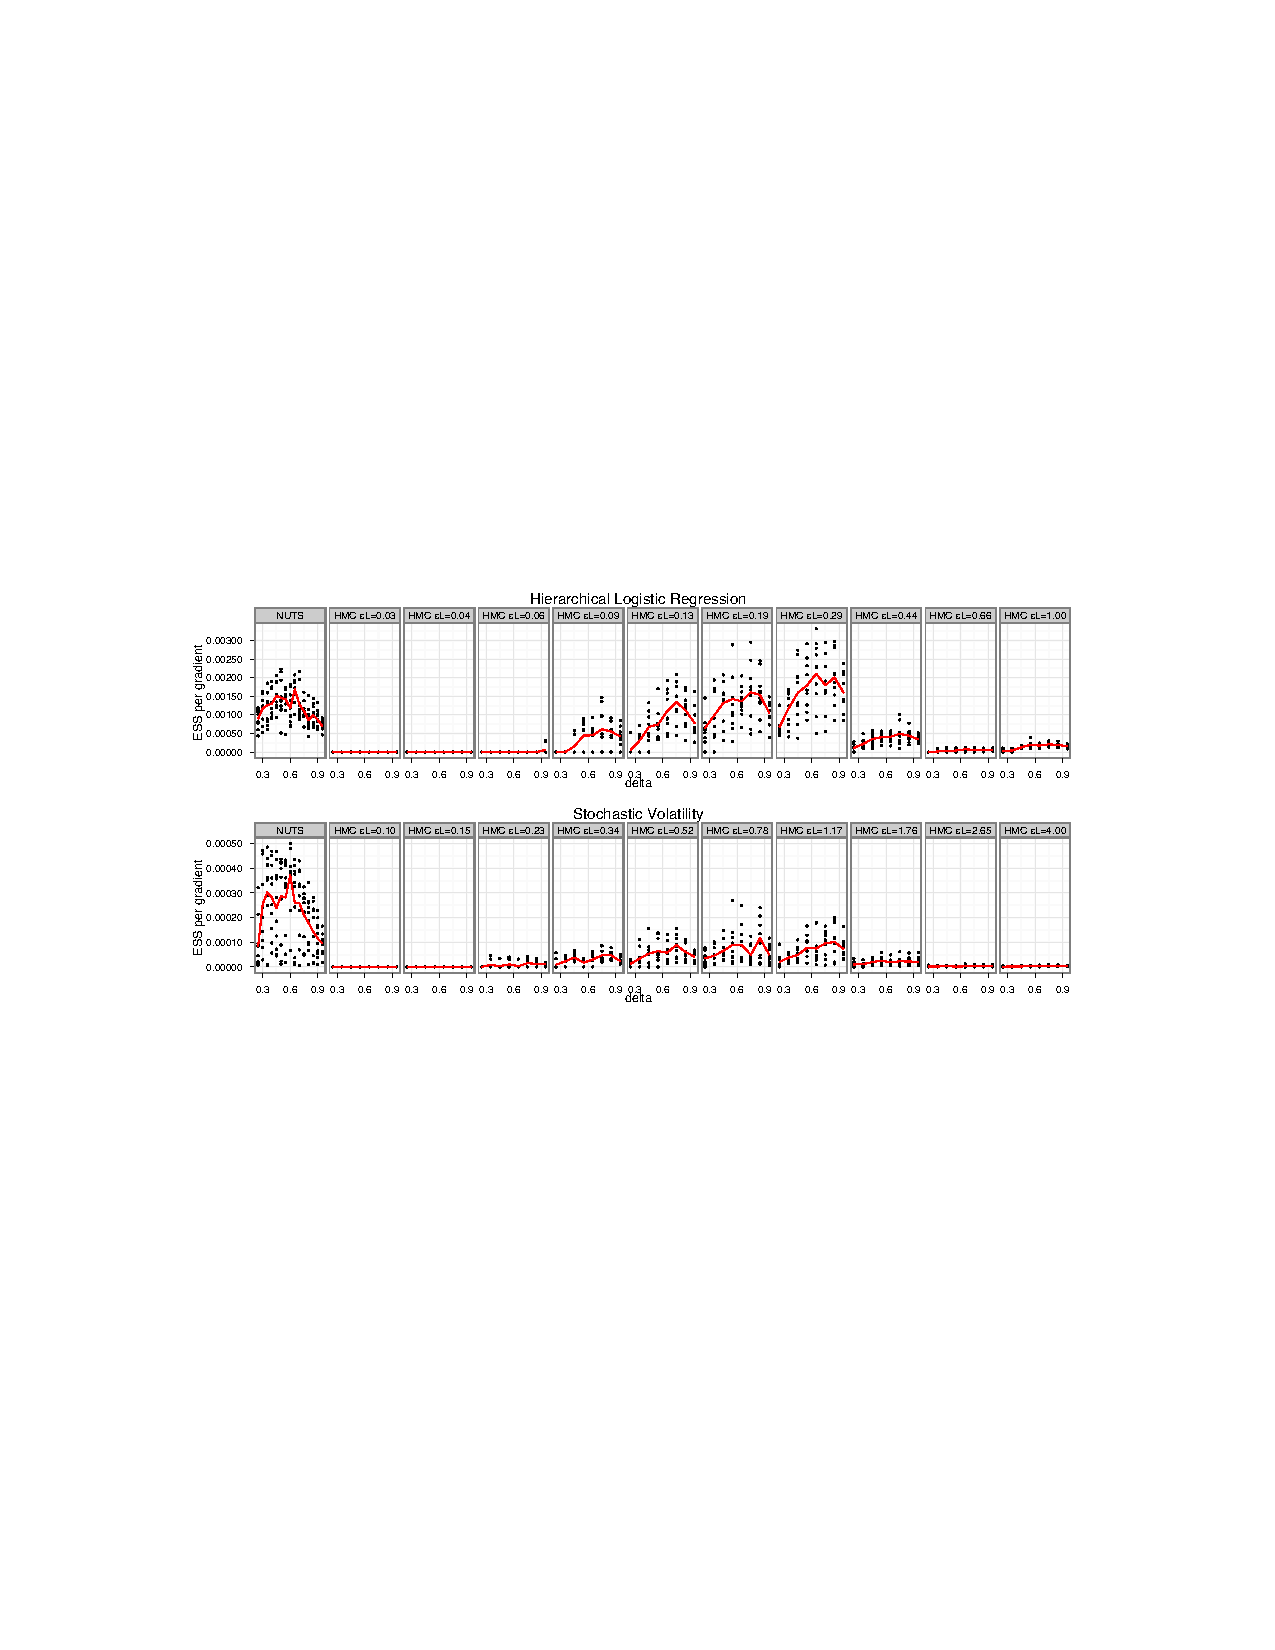
\includegraphics[width=0.9\textwidth]{img/nuts-ess-2.pdf}

{\small
  \begin{itemize}
  \item Hierarchical logistic regression and stochastic volatility
  \item Simulation time $t$ is $\epsilon \ L$, step size ($\epsilon$)
    times number of steps ($L$)
  \item NUTS can beat optimally tuned HMC (latter very expensive)
  \end{itemize}
}


\mypart{Part III}{Under Stan's Hood}

\sld{Euclidean Hamiltonian}

\begin{itemize}
\item \myemph{Phase space}: $q$ position (parameters); \ $p$ momentum
\item \myemph{Posterior density}: $\pi(q)$
\item \myemph{Mass matrix}: $M$
\item \myemph{Potential energy}: $V(q) = -\log \pi(q)$
\item \myemph{Kinetic energy}: $T(p) = \frac{1}{2} p^{\top} M^{-1} p$
\item \myemph{Hamiltonian}:  $H(p,q) = V(q) + T(p)$
\item \myemph{Diff eqs}:
  \[
  \frac{dq}{dt} \ = \  + \frac{\partial H}{\partial p}
  \hspace*{48pt}
  \frac{dp}{dt} \ = \ - \frac{\partial H}{\partial q}
  \]
\end{itemize}

\sld{Leapfrog Integrator Steps}
\begin{itemize}
\item Solves Hamilton's equations by \myemph{simulating dynamics}
  \\
  {\footnotesize (symplectic [volume preserving]; $\epsilon^3$ error per step, $\epsilon^2$ total error)}
\item Given: \myemph{step size} $\epsilon$, \myemph{mass matrix} $M$, \myemph{parameters} $q$
\item \myemph{Initialize kinetic} energy, $p \sim {\sf
    Normal}(0,\mbox{\bf I})$
\item \myemph{Repeat} for $L$ leapfrog steps:
  \begin{eqnarray*}
    p & \leftarrow &
    p - \frac{\epsilon}{2} \, \frac{\partial V(q)}{\partial q}
    \ \ \ \ \ \ \mbox{[half step in momentum]}
    \\[6pt]
    q & \leftarrow &
    q + \epsilon \, M^{-1} \, p
    \ \ \ \ \ \ \ \  \mbox{[full step in position]}
    \\[6pt]
    p & \leftarrow &
    p - \frac{\epsilon}{2} \, \frac{\partial V(q)}{\partial q}
    \ \ \ \ \ \ \mbox{[half step in momentum]}
  \end{eqnarray*}
\end{itemize}


\sld{Reverse-Mode Auto Diff}
\begin{itemize}
\item Eval gradient in (usually small) multiple of function eval time
\begin{subitemize}
\item independent of dimensionality
\item time proportional to number of expressions evaluated
\end{subitemize}
%
\item Result accurate to machine precision (cf. finite diffs)
\item Function evaluation builds up \myemph{expression tree}
\item Dynamic program propagates \myemph{chain rule} in reverse pass
\item Reverse mode computes $\nabla g$ in one
  pass for a function $f : \mathbb{R}^N \rightarrow \mathbb{R}$
\end{itemize}

\sld{Autodiff Expression Graph}
\\
\hspace*{6pt}
\begin{minipage}{0.56\textwidth}
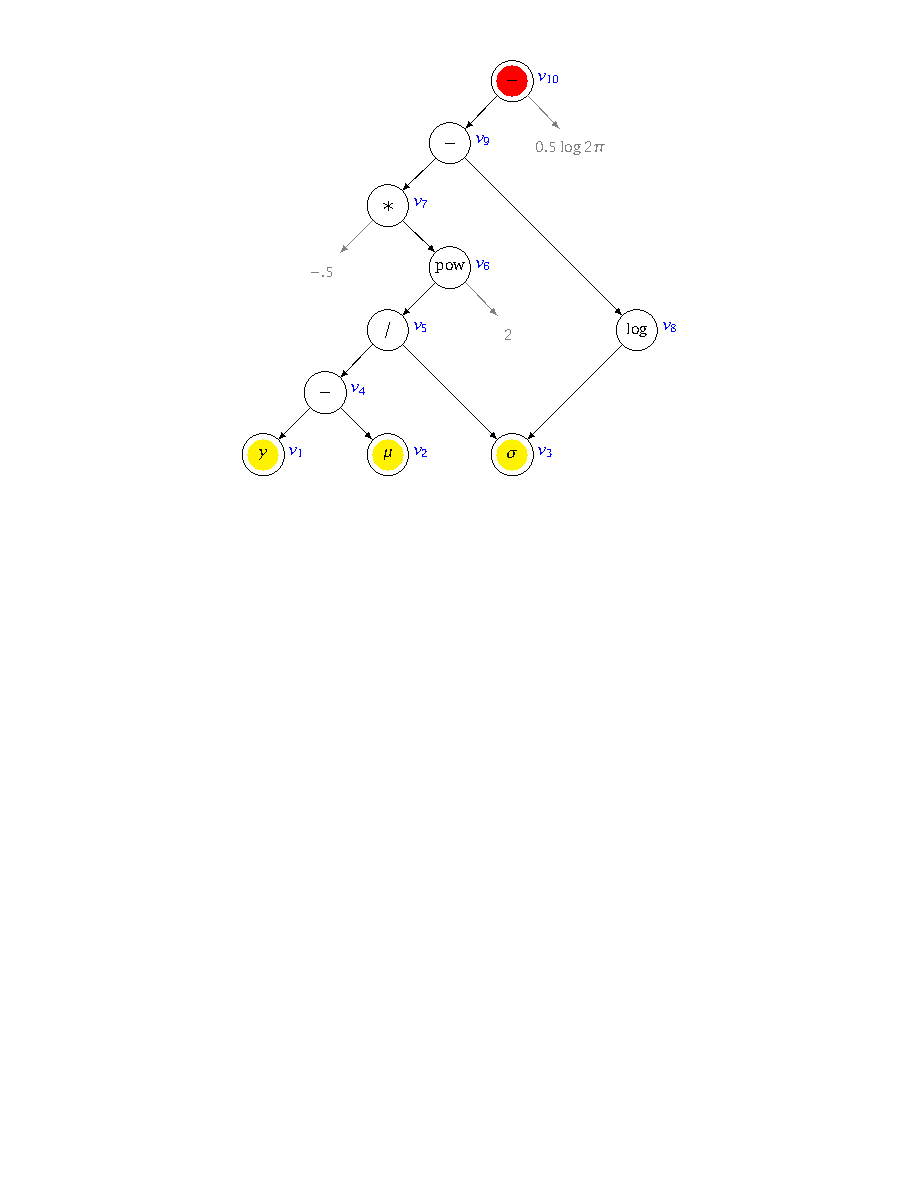
\includegraphics[width=\textwidth]{img/agrad-expression-graph.pdf}
\end{minipage}
\hspace*{-24pt}
\begin{minipage}{0.44\textwidth}
%
\footnotesize
\[
\begin{array}{l}
f(y, \mu, \sigma) 
\\[4pt]
\mbox{ } \ = \ \log \left( \distro{Normal}(y|\mu,\sigma) \right)
\\[4pt]
\mbox{ } \ = \ -\frac{1}{2} \left( \frac{y - \mu}{\sigma} \right)^2
    - \log \sigma
    - \frac{1}{2} \log (2 \pi)
\end{array}
\]
\\
%
\[
\begin{array}{l}
\mbox{ } \hspace*{24pt}
\frac{\partial}{\partial y} f(y,\mu,\sigma)
\\[2pt]
\mbox{ } \hspace*{48pt} = \  -(y - \mu) \sigma^{-2}
\\[8pt]
\mbox{ } \hspace*{24pt} \frac{\partial}{\partial \mu} f(y,\mu,\sigma)
\\[2pt]
\mbox{ } \hspace*{48pt} = \ (y - \mu) \sigma^{-2}
\\[8pt]
\mbox{ } \hspace*{24pt} \frac{\partial}{\partial \sigma} f(y,\mu,\sigma)
\\[2pt]
\mbox{ } \hspace*{48pt} = \ (y - \mu)^2 \sigma^{-3} - \sigma^{-1}
\end{array}
\]
\end{minipage}

\sld{Autodiff Partials}
\begin{center}\footnotesize
\begin{tabular}{c||c|cc}
{\it var} & {\it value} & \multicolumn{2}{|c}{\it partials}
\\ \hline \hline
$v_1$ & $y$ 
\\[2pt]
$v_2$ & $\mu$
\\[2pt]
$v_3$ & $\sigma$
\\[2pt]
$v_4$ & $v_1 - v_2$ & $\partial v_4 / \partial v_1 = 1$ 
                   & $\partial v_4 / \partial v_2 = -1$
\\[4pt]
$v_5$ & $v_4 / v_3$ & $\partial v_5 / \partial v_4 = 1/v_3$
                    & $\partial v_5 / \partial v_3 = -v_4 v_3^{-2}$
\\[4pt]
$v_6$ & $\left(v_5\right)^2$
      & \multicolumn{2}{c}{$\partial v_6 / \partial v_5 = 2 v_5$}
\\[4pt]
$v_7$ & $(-0.5) v_6$ & \multicolumn{2}{c}{$\partial v_7 / \partial v_6
                                          = -0.5$}
\\[4pt]
$v_8$ & $\log v_3$ & \multicolumn{2}{c}{$\partial v_8 / \partial v_3 = 1/v_3$}
\\[4pt]
$v_9$ & $v_7 - v_8$ & $\partial v_9 / \partial v_7 = 1$
                    & $\partial v_9 / \partial v_8 = -1$
\\[4pt]
$v_{10}$ & $v_9 - (0.5 \log 2\pi)$ 
         & \multicolumn{2}{c}{$\partial v_{10} / \partial v_9 = 1$}
\end{tabular}
\end{center}

\sld{Autodiff: Reverse Pass}
{\small
\[
\begin{array}{rcl|l}
{\it var} & {\it operation} & {\it adjoint} & {\it result}
\\ \hline \hline
a_{1:9} & = & 0 & a_{1:9} = 0
\\
a_{10} & = & 1 & a_{10} = 1
\\ \hline
a_{9} & {+}{=} & a_{10} \times (1) & a_9 = 1
\\
a_{7} & {+}{=} & a_9 \times (1) & a_7 = 1
\\
a_{8} & {+}{=} & a_9 \times (-1) & a_8 = -1
\\
a_{3} & {+}{=} & a_8 \times (1 / v_3) & a_3 = -1 / v_3
\\
a_{6} & {+}{=} & a_7 \times (-0.5) & a_6 = -0.5
\\
a_{5} & {+}{=} & a_6 \times (2 v_5) & a_5 = -v_5
\\
a_{4} & {+}{=} & a_5 \times (1 / v_3) & a_4 = -v_5 / v_3
\\
a_{3} & {+}{=} & a_5 \times (-v_4 v_3^{-2}) & a_3 = -1 / v_3 + v_5 v_4 v_3^{-2}
\\
a_{1} & {+}{=} & a_4 \times (1) & a_1 = -v_5 / v_3
\\
a_{2} & {+}{=} & a_4 \times (-1) & a_2 = v_5 / v_3
\end{array}
\]
}

\sld{Stan's Reverse-Mode}

\begin{itemize}
\item Easily extensible \myemph{object-oriented} design
%
\item \myemph{Code nodes} in expression graph for primitive functions
\begin{subitemize}
\item requires \myemph{partial derivatives}
\item built-in flexible abstract base classes
\item \myemph{lazy evaluation} of chain rule saves memory
\end{subitemize}
%
\item Autodiff through templated C++ functions
\begin{subitemize}
\item templating on each argument avoids excess promotion
\end{subitemize}
%
\end{itemize}

\sld{Stan's Reverse-Mode (cont.)}
\begin{itemize}
\item Arena-based \myemph{memory management}
\begin{subitemize}
\item specialized C++ \code{operator~new} for reverse-mode variables
\item custom functions inherit memory management through base
\end{subitemize}
\item Nested application to support ODE solver
\end{itemize}

\sld{Stan's Autodiff vs.\ Alternatives}
\vspace*{-4pt}
\begin{itemize}
\item Stan is \myemph{fastest} (and uses least memory)
\begin{subitemize}
\item among open-source C++ alternatives
\end{subitemize}
\end{itemize}
\vspace*{-8pt}
\hfill \hfill
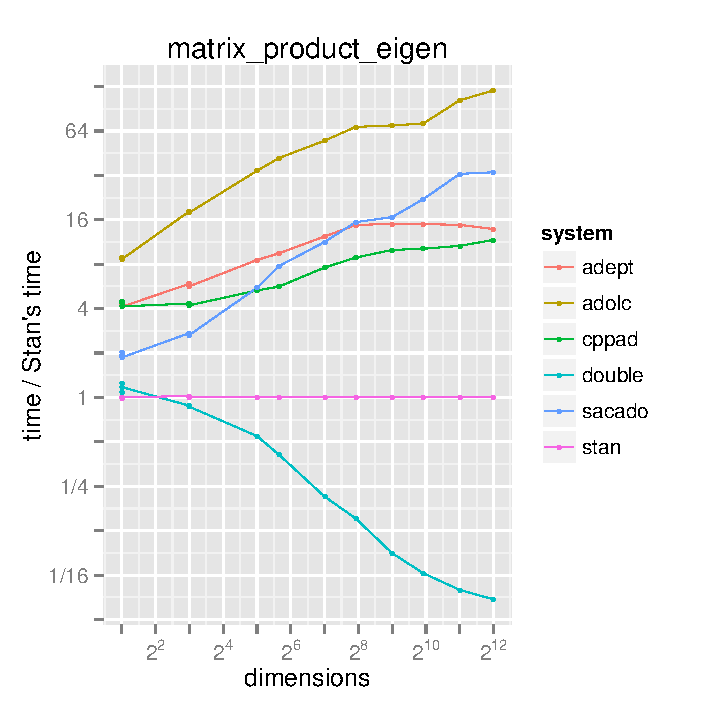
\includegraphics[width=0.48\textwidth]{img/autodiff-eval-matrix-product-eigen.pdf}
\hfill
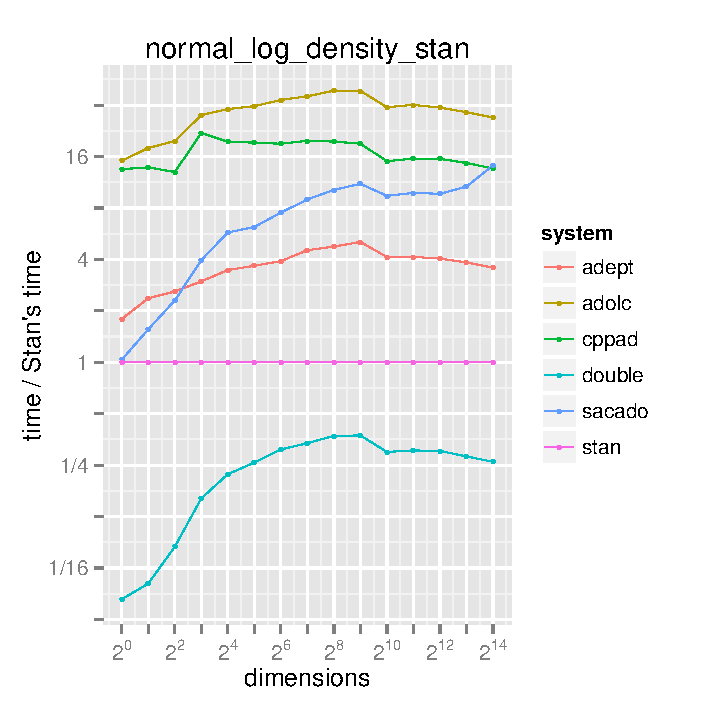
\includegraphics[width=0.48\textwidth]{img/autodiff-eval-normal-density.pdf}
\hfill \hfill




\sld{Forward-Mode Auto Diff}
\begin{itemize}
\item Evaluates expression graph forward from one independent variable
to any number of dependent variables
\item Function evaluation propagates \myemph{chain rule} forward
\item In one pass, computes $\frac{\partial}{\partial x} f(x)$
for a function $f : \mathbb{R} \rightarrow \mathbb{R}^N$ 
\begin{subitemize}
\item derivative of $N$ outputs with respect to a single input
\end{subitemize}
\end{itemize}

\sld{Stan's Forward Mode}
\begin{itemize}
\item Templated scalar type for value and tangent
\begin{subitemize}
\item allows higher-order derivatives
\end{subitemize}
\item Primitive functions propagate derivatives
\item No need to build expression graph in memory
\begin{subitemize}
\item much less memory intensive than reverse mode
\end{subitemize}
\item Autodiff through templated functions (as reverse mode)
\end{itemize}

\sld{Second-Order Derivatives}
%
\begin{itemize}
\item Compute Hessian (matrix of second-order partials)  
\[
H_{i,j} = \frac{\partial^2}{\partial x_i \partial x_j} f(x)
\]
\item Required for Laplace covariance approximation (MLE)
\item Required for curvature (Riemannian HMC)
\item Nest reverse-mode in forward for \myemph{second order} 
\item $N$ forward passes: takes gradient of derivative
\end{itemize}


\sld{Third-Order Derivatives}
\begin{itemize}
\item Compute gradients of Hessians (tensor of third-order partials)
\[
\frac{\partial^3}{\partial x_i \partial x_j \partial x_k} f(x)
\]
\vspace*{-12pt}
\begin{subitemize}
\item Required for SoftAbs metric (Riemannian HMC)
\item $N^2$ forward passes: gradient of derivative of derivative
\end{subitemize}
\end{itemize}

\sld{Jacobians}
%
\begin{itemize}
\item Assume function $f:\mathbb{R}^N \rightarrow \mathbb{R}^M$
\item Partials for multivariate function (matrix of first-order partials)
\[
J_{i,j} = \frac{\partial}{\partial x_i} f_j(x)
\]
\item Required for stiff ordinary differential equations
\begin{subitemize}
\item differentiate is coupled sensitivity autodiff for ODE system
\end{subitemize}
\item Two execution strategies
{\small
\begin{enumerate}
  \item Multiple reverse passes for rows
  \item Forward pass per column (required for stiff ODE)
\end{enumerate}
}
%
%\vfill
%
%\item Order of magnitude faster higher-order autodiff in progress
%\begin{subitemize}
%\item reuse single expression graph
%\item build-in higher-order analytic gradients
%\end{subitemize}
\end{itemize}

\sld{Autodiff Functionals}

\begin{itemize}
\item Functionals map templated functors to derivatives 
\begin{subitemize}
\item fully encapsulates and hides all autodiff types
\end{subitemize}
\item Autodiff functionals supported
  \begin{itemize}\small
  \item gradients: $\bigoh{1}$
  \item Jacobians: $\bigoh{N}$
  \item gradient-vector product (i.e., directional derivative): $\bigoh{1}$
  \item Hessian-vector product: $\bigoh{N}$
  \item Hessian: $\bigoh{N}$
  \item gradient of trace of matrix-Hessian product: $\bigoh{N^2}$
    \\ {\footnotesize (for SoftAbs RHMC)}
  \end{itemize}
\end{itemize}

\sld{Variable Transforms}
\begin{itemize}
\item Code HMC and optimization with $\mathbb{R}^n$ \myemph{support}
\item Transform constrained parameters to unconstrained
  \vspace*{-2pt}
  {\small
    \begin{itemize}
    \item lower (upper) bound: offset (negated) log transform
    \item lower and upper bound: scaled, offset logit transform
    \item simplex: centered, stick-breaking logit transform
    \item ordered: free first element, log transform offsets
    \item unit length: spherical coordinates
    \item covariance matrix: Cholesky factor positive diagonal 
    \item correlation matrix: rows unit length via quadratic stick-breaking
    \end{itemize}
  }
\end{itemize}


\sld{Variable Transforms (cont.)}
\begin{itemize}
\item Inverse transform from unconstrained $\mathbb{R}^n$
\item Evaluate log probability in model block on natural scale
\item Optionally adjust log probability for change of variables
\begin{subitemize}
\item adjustment for MCMC and variational, not MLE
\item add log determinant of inverse transform Jacobian
\item automatically differentiable
\end{subitemize}
\end{itemize}

\sld{Parsing and Compilation}
\begin{itemize}
\item Stan code \myemph{parsed} to abstract syntax tree (AST)
  \\ {\footnotesize (Boost Spirit Qi, recursive descent, lazy semantic
    actions)}
\item C++ model class \myemph{code generation} from AST
  \\ {\footnotesize (Boost Variant)}
\item C++ code \myemph{compilation}
\item \myemph{Dynamic linking} for RStan, PyStan
\end{itemize}

\sld{Coding Probability Functions}
\begin{itemize}
\item \myemph{Vectorized} to allow scalar or container arguments
  \\ {\footnotesize (containers all same shape; scalars broadcast as necessary)}
\item Avoid \myemph{repeated computations}, e.g. $\log \sigma$ in
  \hspace*{-18pt}
  {\small
    \begin{eqnarray*}
      \textstyle \log \, \mbox{\sf Normal}(y | \mu, \sigma)
      & = & \textstyle \sum_{n=1}^N \log \, \mbox{\sf Normal}(y_n | \mu,\sigma)
      \\[4pt]
      & = & \textstyle \sum_{n=1}^N  - \log \sqrt{2\pi} \ - \log \sigma \ -
      \frac{\textstyle y_n - \mu}{\textstyle 2\sigma^2}
    \end{eqnarray*}
  }
\item recursive \myemph{expression templates} to broadcast and cache scalars,
  generalize containers (arrays, matrices, vectors)
\item \myemph{traits} metaprogram to \myemph{drop constants} (e.g., $-\log
  \sqrt{2 \pi}$ or $\log \sigma$ if constant) 
  and calculate intermediate and return types
\end{itemize}


\mypart{}{The End (Section 4)}

\end{document}
